\qquad O Insertion Sort é um algoritmo de ordenação por comparação que
constrói a lista ordenada de forma incremental, um elemento por vez.
Sua lógica é semelhante à forma como uma pessoa organiza cartas de
baralho na mão: a cada nova carta recebida, ela é inserida na posição
correta em relação às cartas que já estão ordenadas.

\qquad O algoritmo percorre o vetor a partir do segundo elemento (índice 1).
A cada iteração, o elemento da posição atual, chamado de \textit{chave},
é comparado com os elementos anteriores, que já se encontram
ordenados entre si. Enquanto houver, à esquerda da chave, elementos
maiores que ela, esses elementos são deslocados uma posição à
frente, abrindo espaço para a chave ser inserida na posição correta.
Esse processo se repete até que todo o vetor tenha sido percorrido,
restando ao final um vetor completamente ordenado em ordem
crescente.

\qquad A seguir apresenta-se a implementação utilizada neste trabalho, em
C++, correspondente à função \texttt{InsertionSort\_versao1}:

\begin{verbatim}
void InsertionSort_versao1(int *vetor, int tamanho) {
    int chave, j;
    for (int i = 1; i < tamanho; i++) {
        chave = vetor[i];
        j = i - 1;
        while (j >= 0 && vetor[j] > chave) {
            vetor[j + 1] = vetor[j];
            j--;
        }
        vetor[j + 1] = chave;
    }
}
\end{verbatim}

\qquad Uma característica importante do Insertion Sort é que seu
desempenho depende diretamente do grau de ordenação da entrada:
quanto mais próxima a entrada já estiver da ordem final, menos
deslocamentos serão necessários durante a execução. Essa
característica é explorada em detalhes na análise de complexidade e
nos resultados experimentais apresentados nas próximas seções deste
capítulo.

\subsection{Teste de Mesa Manual}

\qquad Nesta seção deve ser inserida a digitalização do teste de mesa
manual do Insertion Sort, realizado à mão com um exemplo de entrada
diferente dos exemplos trabalhados em sala de aula, conforme exigido
pelo enunciado do trabalho. Substitua a imagem de exemplo abaixo pela
digitalização (foto ou escaneamento) do teste de mesa manuscrito.

\begin{figure}[htbp]
    \centering
    % Substitua o arquivo abaixo pela digitalizacao do teste de mesa manuscrito
    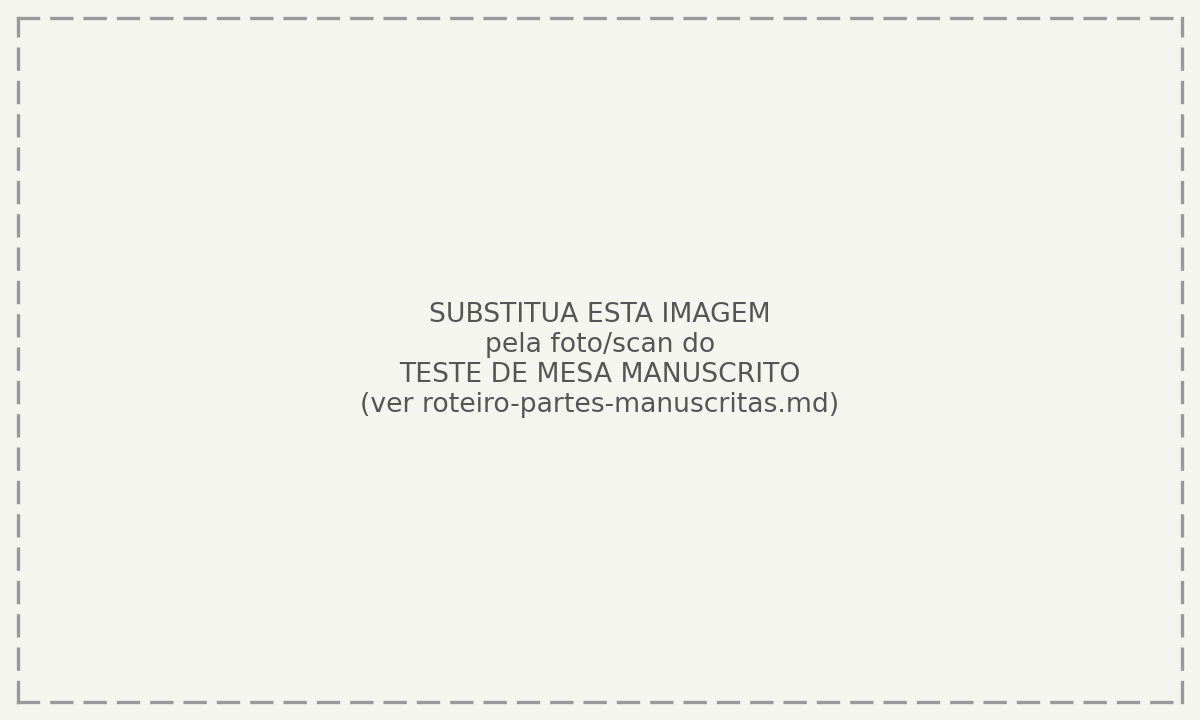
\includegraphics[width=14cm]{Imagens/Insertion Sort/teste_de_mesa.png}
    \caption{Teste de mesa manual do algoritmo Insertion Sort}
    \label{fig:teste_mesa}
\end{figure}
